\documentclass[conference]{IEEEtran}
\IEEEoverridecommandlockouts
\usepackage{cite}
\usepackage{amsmath,amssymb,amsfonts}
\usepackage{algorithmic}
\usepackage{graphicx}
\usepackage{subcaption}
\usepackage{textcomp}
\usepackage{xcolor}
\usepackage{hyperref}
\usepackage{multirow} % tabular
\usepackage{bm}
\def\BibTeX{{\rm B\kern-.05em{\sc i\kern-.025em b}\kern-.08em
    T\kern-.1667em\lower.7ex\hbox{E}\kern-.125emX}}
    
\usepackage{framed}

\begin{document}

\title{Incorporating User Generated Content for Drug Drug Interaction Extraction Based on Full Attention Mechanism
\thanks{This work was supported in part by the Natural Science Foundation of China under Grant 61502071 and Grant 61572094 and in part by the Fundamental Research Funds for the Central Universities under Grant DUT18RC(3)004.}
}

\author{
\IEEEauthorblockN{
Bo Xu\IEEEauthorrefmark{2}\IEEEauthorrefmark{3},
Xiufeng Shi\IEEEauthorrefmark{2}\IEEEauthorrefmark{3},
Zhehuan Zhao\IEEEauthorrefmark{1} \IEEEauthorrefmark{2} \IEEEauthorrefmark{3}\thanks{* Corresponding Author: z.zhao@dlut.edu.cn},
Wei Zheng\IEEEauthorrefmark{4}\IEEEauthorrefmark{5},
Hongfei Lin\IEEEauthorrefmark{4},
Zhihao Yang\IEEEauthorrefmark{4}, 
Jian Wang\IEEEauthorrefmark{4},
and
Feng Xia\IEEEauthorrefmark{2}\IEEEauthorrefmark{3}
}
\IEEEauthorblockA{\IEEEauthorrefmark{2}School of Software, Dalian University of Technology, China}
\IEEEauthorblockA{\IEEEauthorrefmark{3}Key Laboratory for Ubiquitous Network and Service Software of Liaoning, Dalian University of Technology, China}
\IEEEauthorblockA{\IEEEauthorrefmark{4}College of Computer Science and Technology, Dalian University of Technology, China}
\IEEEauthorblockA{\IEEEauthorrefmark{5}College of Software, Dalian JiaoTong University, China}
\\
}

\maketitle

\begin{abstract}
When a patient takes multiple medications simultaneously under the treatment, it is vital for the doctor to fully comprehend all interactions between drugs in the prescription.
Drug drug interaction (DDI) extraction aims to obtain interactions between drugs from biomedical literature automatically.
Nowadays, researchers apply artificial intelligence and natural language processing techniques to perform DDI extraction task.
Existing DDI extraction methods have utilized some kinds of external resources such as biomedical databases or ontologies to offer more knowledge and improve the performance.
However, these kinds of external resources are delayed because of the hardship of updating.
User generated content (UGC) is another sort of external biomedical resource which is up-to-date and can be updated rapidly.
We attempt to utilize UGC resource in our deep learning DDI extraction method to provide more fresh information.
We propose a DDI extraction method that merges UGC information and contextual information together by a new attention mechanism called full-attention.
We conducted a series of experiments on the DDI 2013 Evaluation dataset to evaluate our method.
UGC-DDI outperforms the other state-of-the-art methods and achieves a competitive F-score of 0.712.
\end{abstract}

\begin{IEEEkeywords}
drug drug interaction, drug safety, attention mechanism
\end{IEEEkeywords}

\section{Introduction}
Undoubtedly, it will cause a serious accident if a doctor miscalculates 
potential interactions
between miscellaneous medications which are prescribed to a single patient.
But it is very difficult for doctors to keep pace with frequently updated 
drug interaction knowledge.
Traditionally, physicians acquire new published drug drug interactions (DDIs) 
from two auxiliary information sources:
reading massive biomedical papers to learn DDIs between the lines
or querying DDIs from human-maintained biomedical databases.
Obviously, it is laborious, painful,
and inefficient to read tons of academical papers.
As for searching DDIs from biomedical databases, it seems to be feasible.
But in the consideration of the quantity of the biomedical literature,
it requires a lot of resources to update, maintain and revise a professional database manually.
Apparently, both two of them are not idealistic manners to detect DDIs.

DDI extraction task aims at extracting DDIs from free text of the biomedical domain.
As an illustration, in the following sentence:

\begin{framed}
Because of its primary CNS effect, caution should be used when \textbf{EQUETRO}
is taken with other centrally acting drugs and \textbf{alcohol}.
\end{framed}

\noindent DDI extraction methods attempt to make the prediction of the interaction type,
(such as adverse, recommendation, or no interaction) between
two recognized entities (namely \textbf{EQUETRO} and \textbf{alcohol}, highlighted in bold text).

Much related work of DDI extraction has been done such as FBK-irst 
\cite{chowdhury_fbk-irst:_2013}, WBI-DDI \cite{thomas_wbi-ddi:_2013},
UWM-TRIADS \cite{rastegar-mojarad_uwm-triads:_2013},
Uturku \cite{bjorne_uturku:_2013}, 
and SCNN \cite{zhao_drug_2016}.
These methods utilize artificial intelligence (AI) and natural language processing (NLP) techniques to extract
DDIs.
Some of them introduce external resources to improve the performance of DDI extraction.
WBI-DDI utilizes WordNet lexical database to extract token features.
Uturku sets the presences of words in the DrugBank as a part of features in the 
feature engineering step.
UWM-TRIADS uses a FDA Drug classification dictionary to recognize drugs in the same
drug class during the post-processing phase.
However, external resources used by these methods are from delayed information source such 
as manually-updated databases, ontologies or lexical tools.
These external resources can not be updated timely to catch up with the latest
information.
Many experts are needed to update, review, and revise new items of these external resources.

Compared with these delayed external resources, online User Generated Content (UGC) \cite{krumm_user-generated_2008}
can update more frequently and timely.
As its name suggests, UGC is created by users of online platforms, forums and social media websites.
Considering the count of Internet users, the quantity of UGC is very massive.
UGC is also a more active form of external resources compared with external resources mentioned above \cite{duan_mining_2013}.
Billions of users post text, photos, and videos on the Internet to share their opinions, comments, and experiences every day.
There is lots of information can be mined among these content.
Unfortunately, there are still no research efforts that exploit the external resources with Deep learning approach for DDI extraction. 
To fill this gap, we take the first attempt to investigate the feasibility and advantage of utilizing the UGC in DDI extraction task.

To our knowledge, there is no existing method that utilizes UGC to assist DDI extraction.
Hence, the way to merge UGC with the model is also a challenge.
Recently, self-attention mechanism is a very hot topic in the NLP community.
Experimental results of dozens of papers showed that it performed very well in a lot of NLP tasks
such as machine translation \cite{vaswani_attention_2017} and natural language understanding \cite{shen_disan:_2017}.
Inspired by the self-attention mechanism, we merge UGC with the word embeddings in an attentive way called 
\emph{\textbf{Full-Attention}} to capture the global dependency of every token-UGC document pair comprehensively.
We represent UGC in the form of low-dimensional distributed document embedding vectors.
In order to capture the global dependency of every token-UGC document pair comprehensively,
we build interactions between every single token and every single UGC document by scaled dot product attention.

Based on the ideas we described above, we propose a brand new DDI extraction method named \emph{UGC-DDI}.
UGC-DDI merges UGC embeddings and word embeddings together by the full-attention firstly.
Then the merged vectors are concatenated with the concept embeddings and offset embeddings to generate the final token representations.
At last, token representations are fed into a deep learning based classifier to make predictions of DDI types.
The experimental result shows UGC-DDI outperforms existing methods on DDI 2013 Evaluation dataset.

The rest of this paper is organized as follows.
Section \ref{sec:method} presents the details of the proposed method.
In Section \ref{sec:experiments}, we describe experimental settings and results.
Finally, our conclusion is presented in Section \ref{sec:conclusions}.

\section{Method}
\label{sec:method}

The pipeline of our DDI extraction method is a three-step procedure:

\begin{enumerate}
	\item In the \emph{\textbf{preprocessing}} step, we conduct several kinds of operations to trim and condense raw sentences from DDI 2013 Evaluation dataset.
	\item In the \emph{\textbf{token representation}} step, we merge UGC embeddings and word embeddings to get attention output vectors
	firstly, then concatenate full attention output vectors, concept embeddings, and offset embeddings together to form token representations.
	\item In the \emph{\textbf{classifier}} step, we extract latent features of sentences using a stacked
	two-layer encoder which consists of a Bidirectional Long Short Term Memory (Bi-LSTM) layer and a Transformer layer,
	then make predictions with a Softmax densely-connected neural network layer.
\end{enumerate}

Fig. \ref{fig:pipeline} illustrates the basic pipeline of the UGC-DDI method.

\begin{figure*}[ht]
	\centering
	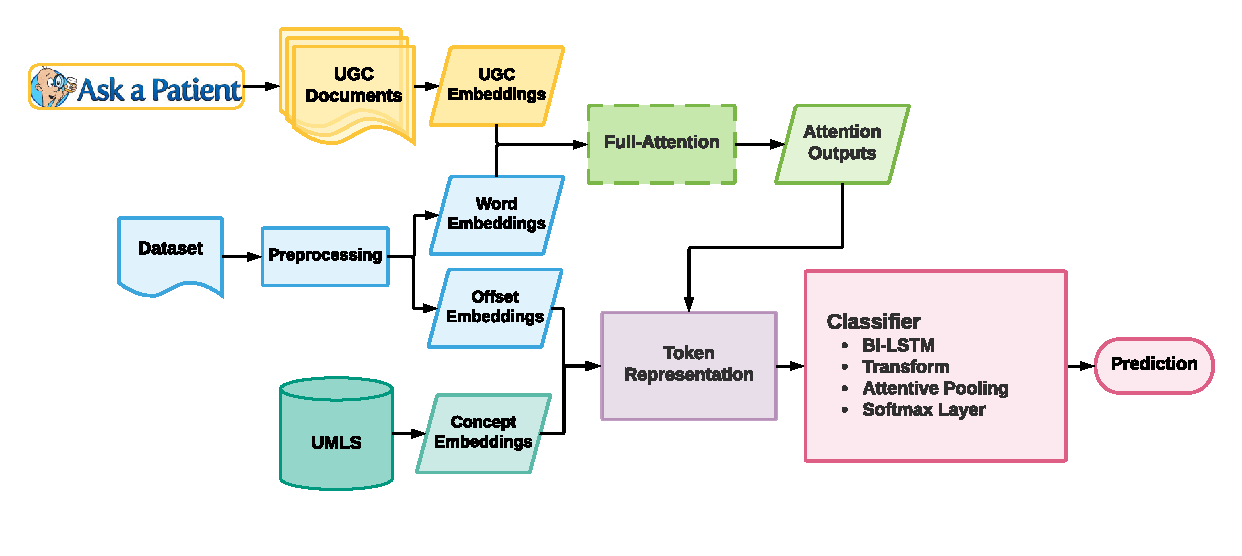
\includegraphics[scale=0.75]{figures/flow-chart-lite}
	\caption{The Pipeline of UGC-DDI method.}
	\label{fig:pipeline}
\end{figure*}

\subsection{Preprocessing}

At the preprocessing step, three kinds of operations are conducted: \emph{Negative Instances Filtering}, 
\emph{Drug Blinding}, and \emph{Tokenization}.

There is no interaction between drugs in negative examples.
In the training dataset of DDI 2013 Evaluation, the positive to negative instances ratio is $1 \colon 5.91$.
Evidently, the dataset is extremely imbalanced.
Imbalanced datasets have been proved that can cause a strong bad influence on the performance of the model \cite{lopez_insight_2013}.
And previous methods \cite{zhao_drug_2016} and \cite{sahu_drug-drug_2017} have verified that negative instance filtering
is a practical operation to relieve the effect of the imbalanced problem.
So firstly, we filter out some negative training examples to balance dataset distribution.

We follow the same negative instance filtering policies of SCNN \cite{zhao_drug_2016} which can be summarized into two rules:

\begin{framed}
\textbf{Rule 1}: If two drugs in a drug pair refer to the same drug,
this pair will be removed under the assumption that the same drug can not interact with itself.
There are two cases to be considered: the first case is two drug names are the same and the second case is one drug is the abbreviation of the other drug.

\bigbreak

\textbf{Rule 2}: If two drugs in a drug pair are in coordinate relations,
this pair will be removed since it is prone to be a false positive \cite{segura-bedmar_lessons_2014}.
\end{framed}

Then, we perform an action called \emph{drug blinding} that replaces concrete drug entity names in sentences with special tokens.
The purpose of drug blinding is to enhance the generalization of the model \cite{liu_drug-drug_2016}.
We replace two drug entity names in every drug pair from the dataset with token \textbf{DURG1} and \textbf{DRUG2},
and replace other drug entity names in the same sentence with token \textbf{DRUGN}.

After the drug blinding step, we tokenize sentences with \emph{GENIA Tagger} \cite{tsuruoka_genia_2006}.
Tokenization converts a sentence into a sequence of tokens.
At this step, we replace numerical tokens with the general token \textbf{NUM} and remove all symbols,
special non-ASCII characters, punctuation marks, and some selected meaningless stop words.

\subsection{Token Representation}

At this step, we generate different kinds of embeddings that contains diverse information firstly,
then concatenate them together to final token representations.\\

\emph{1) Full Attention}

\bigbreak

In full attention phase, we employ full attention mechanism to merge UGC embeddings and word embeddings.

Given a sentence $S = \{t_1, t_2, \dots, t_n\}$ from DDI 2013 Evaluation dataset
which consists of $n$ tokens, we transform this token sequence to corresponding word embeddings
$emb_{\text{word}} = \{ \bm{e_1}, \bm{e_2}, \dots, \bm{e_n} \}$ by a pre-trained word embedding look-up table.
Embedding vector $\bm{e_i} \in \mathbb{R}^{d_{k}}$ in the word embedding sequence contains contextual information of the token $t_i$.

Then we generate UGC embeddings with documents crawled from the website
\href{www.askapatient.com}{\emph{Ask a Patient}}.
Ask a Patient is an online medicine ratings and reviewing forum where patients can
share and compare their medication experiences on various aspects
such as physical or mental feelings, dosage, durations, side effects, etc.
Fig. \ref{fig:askapatient} is a screenshot of Ask a Patient forum which shows patients' reviews of the
\textbf{Chlorpheniramine} which is a drug used in the prevention of the symptoms of allergic conditions.
We use columns \emph{SIDE EFFECTS} and \emph{COMMENTS} in the table to generate UGC documents.
We crawled user reviews of corresponding drug names that appear in the DDI 2013 Evaluation dataset.
Then UGC embeddings are trained with the crawled reviews using document embedding model 
\cite{le_distributed_2014} where each review is regard as a document.
We can map each review to a UGC embedding which is a dense vector.
Every drug name can have multiple comments from different patients,
therefore, a drug name may correspond to multiple UGC embeddings simultaneously.

\begin{figure*}[ht]
	\centering
	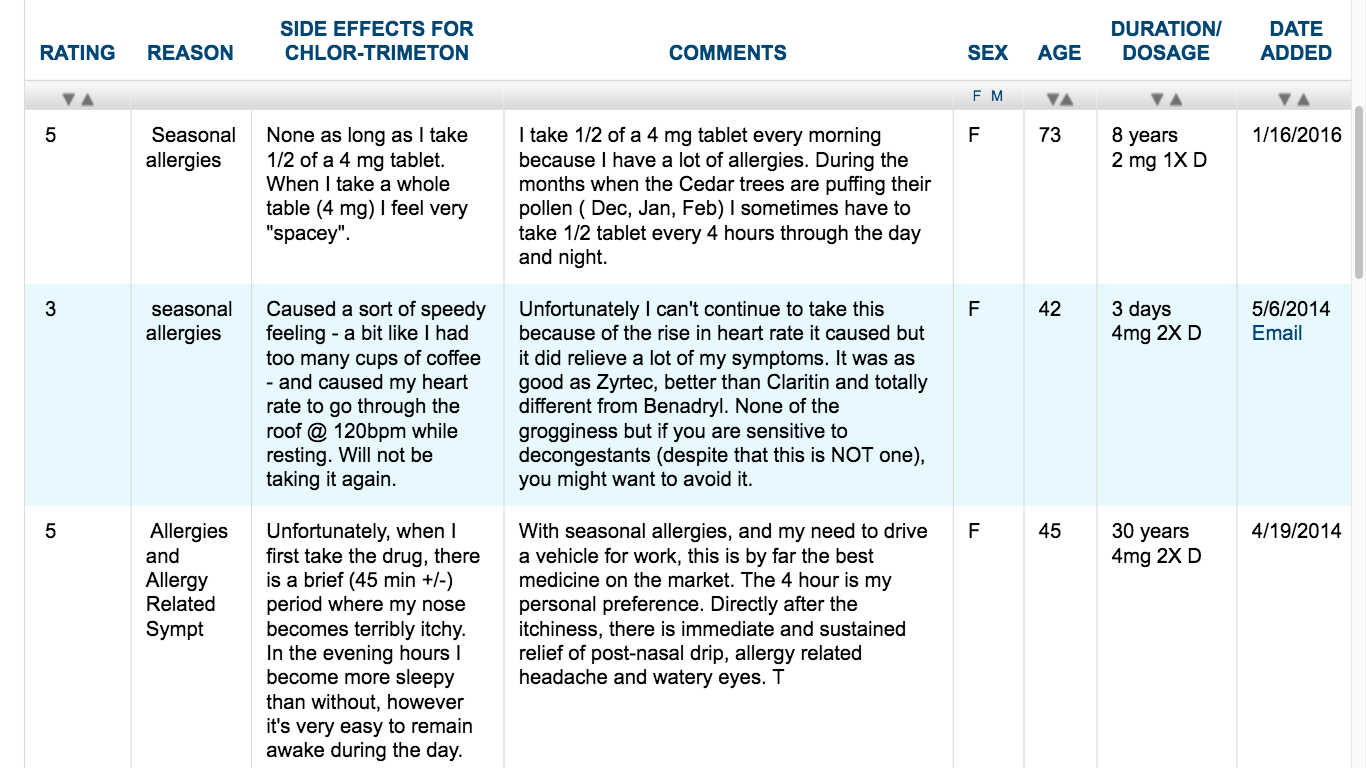
\includegraphics[scale=0.3]{figures/askapatient}
	\caption{Patients' reviews on \textbf{Chlorpheniramine} from Ask a Patient.}
	\label{fig:askapatient}
\end{figure*}

For the sentence $S$, we combine UGC embeddings of two drug names to obtain an unique set $emb_{\text{UGC}} = \{ \bm{u_1}, \bm{u_2}, \dots, \bm{u_g}\}$.
Then, two collections of embeddings, $emb_{\text{word}}$ and $emb_{\text{UGC}}$, are obtained.
Finally, we merge them together by an attentive way called \textbf{\emph{full attention}}.

Full attention is inspired by the self-attention mechanism described in \cite{vaswani_attention_2017}.
We propose full attention based on the \emph{Scaled Product Attention} which is one of core concepts in the self-attention mechanism.
The details of full-attention is shown in (\ref{eq:full-attention}):

\begin{equation}
\label{eq:full-attention}
\bm{a_i} = \text{Attention}(\bm{e_i}, \bm{U_i}) = \text{Softmax}\left ( \frac{\bm{e_i} \bm{U_i^{\top}}}{\sqrt{d_k}} \right ) \bm{U_i}
\end{equation}

\noindent The inputs consist of the word embedding vector $\bm{e_i}$ and a stacked UGC embedding matrix $\bm{U_i} \in \mathbb{R}^{g \times d_k}$ which is the matrix representation of the set $emb_{\text{UGC}}$.
We compute the dot product $\bm{e_i} \bm{U_i^{\top}}$ to get a group of weights between current input token
$t_i$ and its corresponding UGC embeddings.
We use a scaled factor $d_k$ which is the dimension of a UGC embedding vector to reduce the
large-magnitude-growth effect \cite{vaswani_attention_2017}.
Then we use the Softmax function to normalize these scaled weights which stand for correlations between the input token and its UGC embeddings $U_i$.
We can merge these two collections of embeddings depending on computed weights.
Output $\bm{a_i} \in \mathbb{R}^{d_k}$ is a weighted sum of UGC embeddings $\{\bm{u_1}, \bm{u_2}, \dots, \bm{u_g}\}$.
We present a diagram of the full-attention computation procedure in Fig. \ref{fig:full-attention}.

\begin{figure*}[ht]
	\centering
	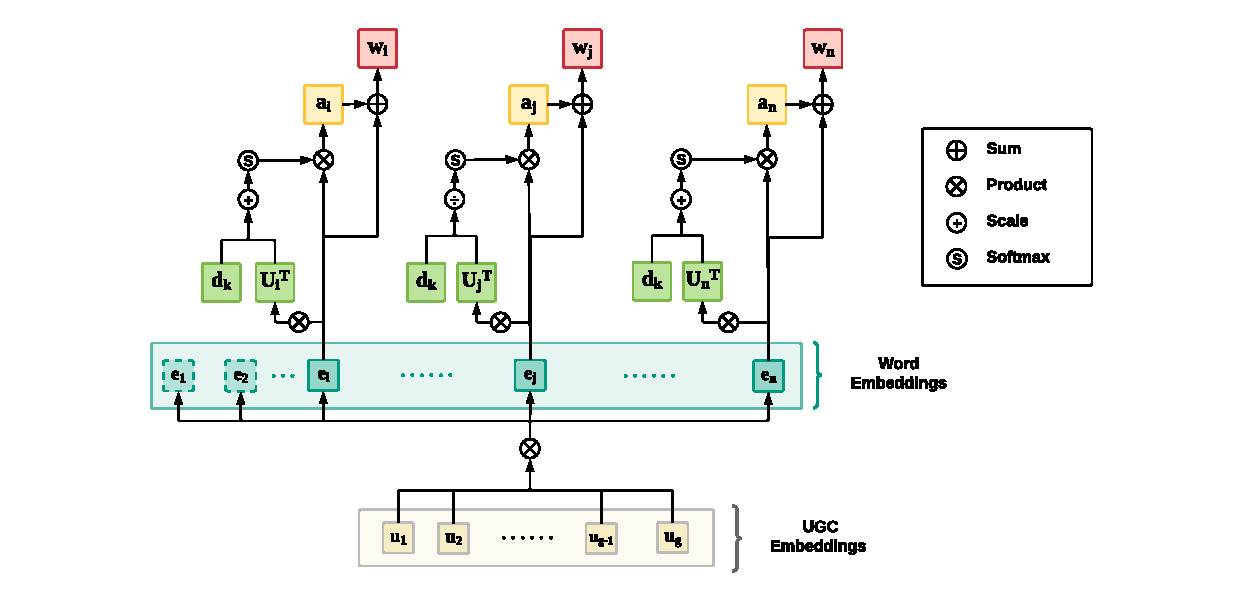
\includegraphics[scale=0.85]{figures/full-attention}
	\caption{The computation procedure of full-attention.}
	\label{fig:full-attention}
\end{figure*}

Full-attention is proposed to compute alignment weights between UGC embeddings and word embeddings,
we combine these two kinds of embeddings according to output weights.
We calculate a scaled dot product of the $\bm{e_i}$ and $\bm{U_i}$ to get a weight distribution
and then normalize it by the Softmax function.
Then, we sum up UGC embeddings with weights computed above
and get an UGC feature vector $\bm{a_i} \in \mathbb{R}^{d_k}$.
Finally, we perform an element-wise summation over it and the original word embedding.

\begin{equation}
\bm{w_i} = \bm{a_i} + \bm{e_i}
\end{equation}

The final output of full-attention $\bm{w_i} \in \mathbb{R}^{d_k}$ combines contextual information from word 
embeddings and external medical knowledge from UGC embeddings.
The computation of full-attention is very intuitive and efficient, no extra parameter is needed.\\

\emph{2) Concept Embeddings}

\bigbreak

Obviously, DDI extraction is an interdisciplinary task that combines biomedical science, computer science, and linguistics.
Due to this nature of DDI extraction, the domain-specific knowledge is also very valuable for this task.
We introduce concept embeddings to add biomedical domain-specific information to the model.
A concept is a biomedical entity such as drugs, proteins, genes, etc.
We use the taxonomy of Unified Medical Language System (UMLS) ontology \cite{bodenreider_unified_2004},
and every concept is assigned a Concept Unique Identifier (CUI).
Concept embeddings are low-dimensional vectors which are learned from the relations between 
concepts and semantics of concepts.
We firstly translate a sentence from a token sequence to a CUI sequence by the \emph{MetaMap} toolkit \cite{aronson_overview_2010}.
Then we map CUIs to corresponding concept embeddings which are trained by the concept embedding model proposed in \cite{de_vine_medical_2014}.
For the sentence $S$, now we have a concept embedding list
$emb_{\text{concept}} = \{ \bm{p_1}, \bm{p_2}, \dots, \bm{p_n}\}$.
Concept embedding list and token sequence have the same length \cite{wang_ontology-based_2017}.\\

\emph{3) Offset Embeddings}

\bigbreak

Offset embeddings can supply distance information between the current token and two drug 
entities.
We calculate distances of tokens from the current token to the two drugs, i.e. \textbf{DRUG1} and \textbf{DRUG2}, in the drug pair respectively.
Then we convert two distances into two offset embeddings by an dynamic offset lookup table.
The basic idea of offset embeddings is that adjacent tokens make more contributions to the final predictions.
So we want the model to give more concentration to nearby words of drug entities.

For the token $t_i$ in the sentence $S$, we concatenate the attention output vector $\bm{w_i}$,
the concept embedding $\bm{p_i}$ and the offset embeddings $\bm{o1_i} \in \mathbb{R}^{d_o}$,
$\bm{o2_i} \in \mathbb{R}^{d_o}$ together to generate the final token representation $\bm{x_i} \in \mathbb{R}^{d_k + d_k + 2 \times d_o}$:

\begin{equation}
	\bm{x_i} = \left [ \bm{w_i} +\!\!\!\!+\, \bm{p_i} +\!\!\!\!+\, \bm{o1_i} +\!\!\!\!+\, \bm{o2_i} \right ].
\end{equation}

\subsection{Classifier}
In this step, we extract latent features of sentences by a deep learning encoder and make predictions of DDI type with a Softmax densely-connected neural network.

We build a stacked two-layer encoder consists of a Bi-LSTM layer and a Transformer Layer.
Bi-LSTM \cite{hochreiter_long_1997, schuster_bidirectional_1997} is a powerful sentence embedding architecture \cite{lin_structured_2017}, it has been applied to extensive NLP tasks such as
speech recognition \cite{sak_long_2014}, sequence tagging \cite{huang_bidirectional_2015}, dependency parsing \cite{kiperwasser_simple_2016}, and event detection \cite{feng_language-independent_2018}
as an encoder.
So we choose Bi-LSTM to be one layer of our stacked encoder.
Given a token representation list $X_S = \{ \bm{x_1}, \bm{x_2}, \dots, \bm{x_n} \}$  of sentence $S$, we calculate two collections
of outputs named hidden states:
forward hidden states $\overrightarrow{\bm{h}} = \{\overrightarrow{\bm{h}_1}, \overrightarrow{\bm{h}_2}, \dots, \overrightarrow{\bm{h_n}}\}$
and backward hidden states $\overleftarrow{\bm{h}} = \{\overleftarrow{\bm{h}_1}, \overleftarrow{\bm{h}_2}, \dots, \overleftarrow{\bm{h_n}}\}$.
We concatenate them to get the final output of Bi-LSTM layer:

\begin{equation}
\bm{h_i} = \left [ \overrightarrow{\bm{h_i}} +\!\!\!\!+\,  \overleftarrow{\bm{h_i}} \right ]
\end{equation}

After the Bi-LSTM layer, a Transformer layer which is described in \cite{vaswani_attention_2017} follows.
We append the Transformer layer at this position because Transformer model is more efficient and can capture more global dependency.
The Transformer Model we use includes $N$ Transformer blocks, and between the blocks we connect these blocks with residual connections and layer normalizations.
After the process of the Transformer model, we get a list of token features $\bm{h'} = \{ \bm{h'_1}, \bm{h'_2}, \dots, \bm{h'_n} \}$.
In practice, we stack the token feature list as a matrix $\bm{\text{H}} \in \mathbb{R}^{n \times d_h}$, $d_h$ is the dimension of a single token feature vector.

We use an attentive pooling method to generate sentence feature vectors.
Given the token feature matrix $\bm{H}_S \in \mathbb{R}^{n \times d_h}$ of sentence $S$, we first calculate a token weights vector $\bm{v_S'} \in \mathbb{R}^{n}$:

\begin{equation}
\bm{v}_S = \tan \left ( W H_S^{\top} + \bm{b} \right ),
\end{equation}

\begin{equation}
\bm{v'}_S = Softmax \left (  \bm{v}_S^{\top} \cdot \bm{w_v} \right ),
\end{equation}

\noindent
$W \in \mathbb{R}^{d_h \times d_h}$, $\bm{b} \in \mathbb{R}^{d_h}$, and $\bm{w_v} \in \mathbb{R}^{d_h}$ are all learnable parameters.

Then we compute the final sentence embedding $\bm{emb_{\text{S}}} \in \mathbb{R}^{d_h}$ which is a weighted sum of token features:

\begin{equation}
\bm{emb_{\text{S}}} = \sum_{i=0}^{n} {(\bm{v'}_S)_i \times (\bm{h'}_S)_i}
\end{equation}

After getting the sentence embedding vector, we feed it into a Softmax layer to make predictions:

\begin{equation}
\bm{DDI_S} = Softmax \left ( W_C \times \bm{emb_{\text{S}}}^{\top} + \bm{b_C} \right ),
\end{equation}

where the output $\bm{DDI_S} \in \mathbb{R}^C$ is a DDI type distribution, $C$ is the count of 
the DDI types.
The weight $W_C \in \mathbb{R}^{C \times d_h}$ and the bias $\bm{b_C} \in \mathbb{R}^C$ are trainable parameters.

\section{Experiments}
\label{sec:experiments}

We built our method with Python and Keras deep learning library \cite{chollet_keras_2015} running on the top of 
TensorFlow \cite{girija_tensorflow:_2016} backend.
We trained our model on a NVIDIA TITAN Xp graphic card whose frame buffer size is 12GB.

\subsection{Dataset Description And Evaluation Metrics}

We evaluated our method on the DDI 2013 Evaluation datasets \cite{segura-bedmar_semeval-2013_2013}.
The datasets consist of $27, 792$ and $5, 716$ drug pairs in the training set and the test set, respectively.
There is one kind of $negative$ label and four types of positive DDI labels: $advise$, $mechanism$, $int$, and $effect$. 
As we mentioned before, we filtered out some negative instances in the preprocessing step.
We list the label type distribution before and after the negative instance filtering phase in the Table \ref{table:neg_filter}.

We used official evaluation metrics, precision (P), recall (R), and F-score (F) to measure the performance of our DDI extraction method.

\begin{table}
\caption{Label distribution before and after the negative instance filtering phase.}
\label{table:neg_filter}
\normalsize
\begin{center}
\begin{tabular}{ccccc}
\hline
\multirow{2}*{Class} &\multicolumn{2}{c}{Training Set} & \multicolumn{2}{c}{Test Set} \\ \cline{2-5}
& Before & After & Before & After \\ \hline
\emph{negative} & 23772 & 8987 & 4737 & 2049\\ 
\emph{advise} & 826 & 814 & 221 & 221 \\ 
\emph{effect} & 1687 & 1592 & 360 & 357\\ 
\emph{mechanism} & 1319 & 1260 & 302 & 301\\ 
\emph{int} & 188 & 188 & 96 & 92 \\
ratio & 1:5.91 & 1:2.33 & 1:4.83 & 1:2.11 \\ 
Total & 27792 & 12841 & 5716 & 3020 \\ \hline
\end{tabular}
\end{center}
\end{table}

\subsection{Hyper-parameters and training strategies}

UGC embeddings, word embeddings and concepts embeddings used in our method are all pre-trained and their dimensions are all $200$.
Word embeddings \cite{moen_distributional_2013} were induced from PubMed and PubMed Central (PMC) texts by the Word2vec model \cite{mikolov_distributed_2013, mikolov_efficient_2013}.
We updated word embeddings during the training process.
In contrast, concept embeddings and UGC embeddings stayed static.
UGC embeddings are trained by the gensim toolkit\cite{rehurek_software_2010}.
DRUG1 offset embeddings and DRUG2 offset embeddings shared the same embedding look-up table whose dimension is $20$.
Offset embedding vectors were initialized randomly and were also updated dynamically.

The hidden state dimension is $250$ in our Bi-LSTM encoder.
Our Transformer encoder consists of $N=4$ Transformer self-attention blocks.
The feedforward dimension is $512$ and the count of heads of multi-head self-attention computation 
in the Transformer encoder is $5$ which is the same as the count of our DDI types
(one negative type and four positive types).
To overcome the overfitting problem, we used the dropout technique in our classifier with a drop rate value $0.5$.
We also used several L1-L2 regularizers \cite{ng_feature_2004}  inside our model, the weight decay value was $0.08$.
We trained our model with an Adam optimizer \cite{kingma_adam:_2014}, the learning rate we used was $0.0004$, other hyper-parameters of optimizers were all default values. Our training batch size was $128$ and testing batch size was $64$,.
The zero-masking strategy was used to train on variance-length sequences.
We list all of our hyper-parameters in Table \ref{table:hypers}.

\begin{table}
\caption{Hyper-parameter list}
\label{table:hypers}
\centering
\begin{tabular}{ll}
\hline
 Name & Value\\ \hline
UGC embedding dimension & 200\\
 word embedding dimension & 200\\
 concept embedding dimension & 200\\
 offset embedding dimension & 20\\
 hidden state dimension & 250\\
 feedforward dimension of Transformer & 512 \\ 
 head count of Transformer & 5 \\  
 block count of Transformer & 4 \\  
 weight decay & 0.08\\
 dropout probability & 0.5 \\
 training batch size & 128 \\
 test batch size & 128 \\
 Adam-learning rate & 0.004\\
 Adam-$\beta-1$ & 0.9\\
 Adam-$\beta-2$ & 0.999\\
 Adam-$\epsilon$ (epsilon) & 1e-08\\
 Adam-learning rate decay & 0\\
 \hline
\end{tabular}
\end{table}

\subsection{Experimental Result}

Table \ref{table:class_metric} presents the evaluation results of every single DDI type.
As can be seen, ``int'' DDI type only achieves an F-score of $0.4545$ which is much lower than that of other three DDI types.
It obtains a recall of $0.3125$ that causes the lowest F-score.
``int'' DDI type is assigned when the sentence simply states that an interaction occurs
and does not provide any information about the interaction \cite{segura-bedmar_semeval-2013_2013}.
Due to the ambiguous meaning of the ``int'' DDI type, it is error prone to misclassified instances to other specific DDI types.
The ``mechanism'' type achieves the highest F-score, this is probably because ``mechanism'' describes a pharmacokinetic mechanism.
Pharmacokinetic means that the effects of one drug are changed by the presence of another drug at its site of action which is relatively not easy to confuse.

\begin{table*}
\caption{Detailed evaluation metrics of DDI-UGC.}
\normalsize
\label{table:class_metric}
\begin{center}
\begin{tabular}{cccccccc}
\hline
& TP & FP & FN & Total &P & R & F \\\hline
mechanism &  230 & 69 & 72 & 302 & 0.769 & 0.762 & 0.765\\
effect &  240 & 101 & 120 & 360 & 0.704 & 0.667 & 0.685\\
advise &  154 & 28 & 67 & 221 & 0.846 & 0.697 & 0.764 \\
int &  30 & 6 & 66 & 96 & 0.833 & 0.312 & 0.455\\
classification & 654 & 204 & 325 & 979 & 0.762 & 0.668 & 0.712\\
\hline
\end{tabular}
\end{center}
\end{table*}

\bigbreak
\emph{1) Performance comparison}
\bigbreak

Evaluation metrics comparison with other state-of-the-art methods are showed in the Table \ref{table:comp}.
The highest values of every metric are highlighted in bold text.
Our methods achieved the highest F-score of 0.712 and the highest recall of 0.668 in the comparison.

\begin{table}
\caption{Performance comparison between methods}
\normalsize
\label{table:comp}
\centering
\begin{tabular}{cccc}
\hline
 Methods & P & R & F \\ \hline
 UTurku \cite{bjorne_uturku:_2013} & 0.732 &  0.499 &  0.594\\
 WBI-DDI \cite{thomas_wbi-ddi:_2013} & 0.642 &  0.579 &  0.609 \\
 FBK-irst \cite{chowdhury_fbk-irst:_2013} &  0.646 & 0.656 & 0.651\\
 Kim \emph{et al.} \cite{kim_extracting_2015} & --- & --- &  0.670\\
  SCNN$^1$ \cite{zhao_drug_2016} &  0.691 & 0.651 & 0.670\\
 SCNN$^2$ \cite{zhao_drug_2016} &  0.725 & 0.651 & 0.686\\
 Joint AB-LSTM \cite{sahu_drug-drug_2017} &  0.745 & 0.645 & 0.694\\
 DCNN \cite{liu_dependency-based_2016} & \textbf{0.772} & 0.644 & 0.702 \\
 Our method without UGC resource & 0.756 & 0.656 & 0.702 \\
 UGC-DDI & 0.762 & \textbf{0.668} & \textbf{0.712} \\\hline
\end{tabular}
\end{table}

The preceding four methods in Table \ref{table:comp} UTurku, WBI-DDI, FBK-irst, and Kim et al. are all support vector machine (SVM) based DDI extraction methods.
One significant drawback of SVM based models is that they usually utilize complex human-selected lexical or
syntactical features to form representations of sentences or tokens.
For examples, Kim et al. which performs best among SVM based DDI extraction methods uses a linear SVM classifier
with a rich set of lexical and syntactic features to extract DDI.
FBK-irst utilize a hybrid kernel SVM classifier with syntax tree and dependency tree features.

SVM based methods are all highly dependent on the external lexical tools such as part-of-speech tagger,
chunk tagger, and dependency parser to analyze text and construct features from the processing output.
Errors from the external lexical tools can propagate to the DDI extraction method through the pipeline \cite{jiao_chinese_2018}.
Selecting features manually is laborious and time-consuming compared with deep learning latent features.
From another perspective, human-selected features may also perform poor on generalization.
Compared with FBK-irst and Kim et al., UGC-DDI learns high-level latent features automatically from the deep learning network encoder
and the attentive pooling method.
It also does not depends on any external lexical or syntactical analyzer to generate features.
However, UGC-DDI achieves an F-score of $0.712$ which is higher than that of FBK-irst and Kim et al. by $0.061$ and $0.042$, respectively.

Remaining methods in Table \ref{table:comp} are all deep learning based methods.
They can be categorized into two types: convolutional neural network based methods and bidirectional long short-term memory (Bi-LSTM) network based methods.
SCNN \cite{zhao_drug_2016} is a syntax convolutional neural network based DDI extraction method.
In SCNN, a novel word embedding, syntax embedding, is proposed to employ syntactical information of a sentence.
SCNN also employs many hand-crafted features to improve the performance of DDI extraction that makes the extraction process more complicated.
Compared with SCNN, UGC-DDI extracts no traditional feature but achieves a higher F-score, $0.712$ vs. $0.686$.

Joint AB-LSTM is a bidirectional long short-term memory based DDI extraction method.
It joins two separate bidirectional long short-term memory network, B-LSTM and AB-LSTM to generate a sentence embedding.
B-LSTM and AB-LSTM utilize two different pooling methods max poling and attentive pooling in their own model to unify token embeddings.
Instead of two independent Bi-LSTM networks, UGC-DDI utilize a stacked two-layer encoder inside the classifier,
two encoder layers can share the information and communicate with each other.
Besides the model architecture, UGC-DDI also utilizes domain-specific knowledge such as UGC embeddings and concept embeddings
in the procedure of DDI extraction.
Compared with Joint AB-LSTM, UGC-DDI achieves a higher F-score ($0.712$ vs. $0.694$) with a richer set of information sources.

\bigbreak
\emph{2) UGC feature analysis}
\bigbreak

UGC external biomedical resource is a core information source in our UGC-DDI method.
To evaluate the improvement made by the external UGC resource, we compared the metrics of our method
with and without UGC embeddings in Fig. \ref{fig:ugc-exp}.
We conduct an extra comparison experiment which concatenates the word embeddings, concept embeddings and two offset embeddings directly as token representations.
Other model components such as encoders and attentive pooling layer are all the same as the UGC-DDI method settings.
We can see that the F-score of UGC-DDI method increases more rapidly and climb to a highest peak in a extremely short period (94th epoch in about half an hour).
Although the method without UGC resource does not get a better performance compared with UGC-DDI,
it gains a relatively good performance compared with other existing methods, either SVM based methods or deep learning based methods.
As we mentioned before, UGC embeddings stayed static during the training procedure.
And the full-attention mechanism does not add new parameters into the model, it just merge UGC embeddings and word embeddings based on their
scale dot products and summations.
No extra training cost is needed compared with the method without UGC resource.
Compared with directly concatenating UGC embeddings with word embeddings or other non-attentive manner,
full-attention does not increase the dimension of the token representation and enrich the information offered to the classifier.
This advantage also control the magnitude of parameters of the whole network and prevent suffering from the overfitting issue.

The F-score of the method without the UGC resource is $0.702$ and the F-score is improved by $1\%$ with the utilization of the UGC resource.

%\begin{figure}[ht]
%	\centering
%	\begin{subfigure}[b]
%		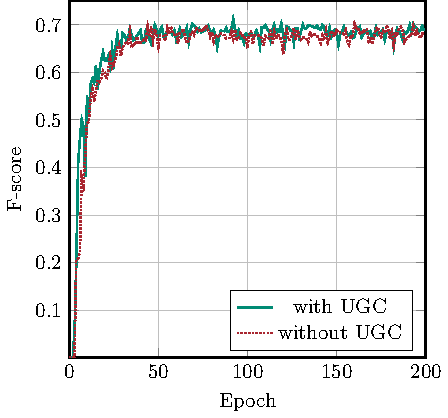
\includegraphics[scale=0.5]{figures/ugc-exp-f.pdf}
%	\end{subfigure}
%	\label{fig:ugc-exp}
%\end{figure}

\begin{figure*}[htb]
    \centering
    \begin{subfigure}[b]{\textwidth}
    \centering
        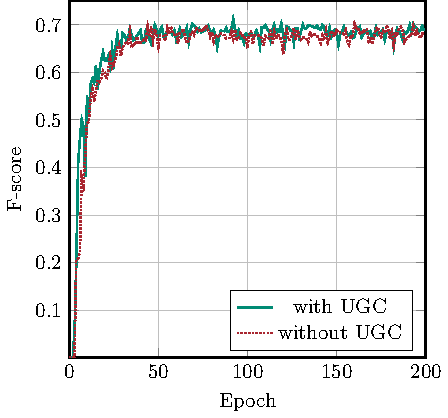
\includegraphics[scale=0.7]{figures/ugc-exp-f}%
        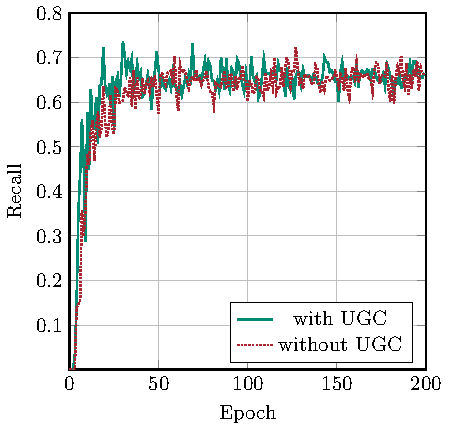
\includegraphics[scale=0.7]{figures/ugc-exp-r}
    \end{subfigure}
    \vskip\baselineskip
    \begin{subfigure}[b]{\textwidth}
    \centering
        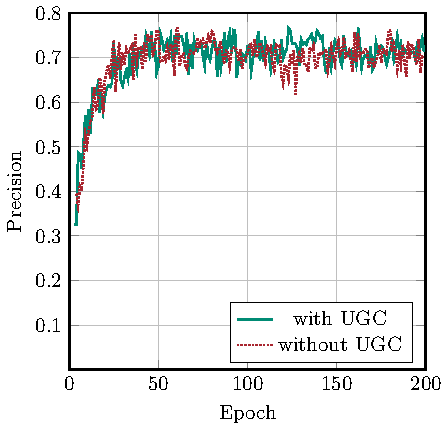
\includegraphics[scale=0.7]{figures/ugc-exp-p}%
        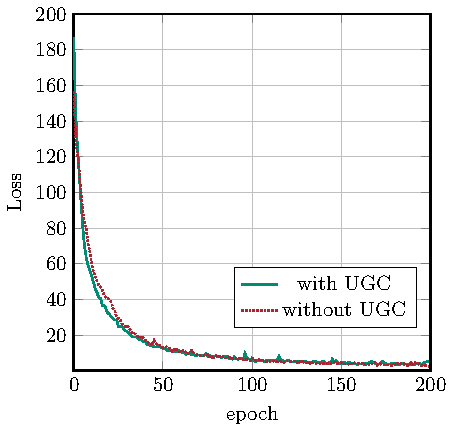
\includegraphics[scale=0.7]{figures/ugc-exp-loss}
    \end{subfigure}
    \caption{Metrics comparison of methods with and without UGC resource during the training.}
    \label{fig:ugc-exp}
\end{figure*}

\section{Conclusions}
\label{sec:conclusions}

In this study, we proposed a novel methods namely UGC-DDI to extract DDI from biomedical literature automatically.
We merge user generated content with local contextual information by full-attention mechanism to provide rich and fresh knowledge.
User generated content are offered in the form of low-dimension embedding vectors.
Attention outputs are concatenated with concept embeddings and entity offset embeddings together to be the input of the deep learning classifier of our method.
The experimental result shows that our method gains the highest evaluation metrics values.

\bibliographystyle{IEEEtran}
\bibliography{UGC-DDI}

\end{document}
